\documentclass[aspectratio=169,11pt]{beamer}
% Shared preamble for the CogLean decks.
% Build the slides alone, or with speaker notes (see the Makefile):
%   pdflatex deck.tex                                   -> slides
%   pdflatex -jobname=deck-notes "\def\withnotes{}\input{deck.tex}"  -> slides + notes
\usetheme{default}
\usecolortheme{seahorse}
\setbeamertemplate{navigation symbols}{}
\setbeamertemplate{footline}[frame number]
\setbeamerfont{note page}{size=\small}
\ifdefined\withnotes
  \setbeameroption{show notes}
\fi
\usepackage[T1]{fontenc}
\usepackage{lmodern}
\usepackage{booktabs}
\usepackage{amsmath,amssymb}
\usepackage{tikz}
\usetikzlibrary{positioning,arrows.meta,shapes.misc}
\tikzset{
  box/.style={draw, rounded corners, align=center, minimum height=8mm, inner sep=4pt, fill=blue!6},
  arr/.style={-{Stealth[length=2mm]}, thick}
}
\newcommand{\code}[1]{\texttt{#1}}
\newcommand{\has}{\textbf{has}}
\newcommand{\lacks}{\textcolor{red!70!black}{lacks}}
\newcommand{\never}{\textcolor{red!70!black}{\textbf{never}}}
\newcommand{\canhold}{can hold}


\title{Problem solving, proved}
\subtitle{Means-ends analysis, impasses, and the bugs of multi-column addition}
\author{Jeff Shrager}
\date{October 2026}

\begin{document}

\begin{frame}
  \titlepage
\end{frame}
\note{
This talk brings problem solving into CogLean, in the tradition that runs from GPS to Soar. I'll set up one problem space, run two control regimes over it, means-ends analysis and a decision cycle with impasses, and use multi-column addition as the domain. Three results: the problem solver computes exactly what the multi-digit model's column backup computed, so it can replace it; GPS works the units column first though nothing tells it to; and deleting the carry rule produces impasses whose repairs are the classic addition bugs, one bug per repair.
}

\begin{frame}{A problem space}
  \begin{itemize}
    \item \textbf{States} and \textbf{operators}; each operator has \textbf{preconditions} and an \textbf{effect} (Newell \& Simon).
    \item An effect is a \emph{distribution} over states, so an operator can include a probabilistic process, such as retrieving a fact from memory.
    \item One space, two control regimes:
    \begin{itemize}
      \item \textbf{Means-ends analysis} (GPS): goals as differences, subgoals on unmet preconditions, backtracking.
      \item \textbf{A decision cycle with impasses} (repair theory; Soar): rules propose an operator; a violated precondition is an impasse, repaired locally.
    \end{itemize}
  \end{itemize}
\end{frame}
\note{
A problem space has states and operators, and each operator has preconditions and an effect. In CogLean an effect is a probability distribution over states, so an operator can include a probabilistic process, such as retrieving an arithmetic fact from memory. Over one space we can run two control regimes. Means-ends analysis, the heart of GPS, works from differences between the state and the goal. And a decision cycle, where rules propose an operator and a violated precondition is an impasse that has to be repaired: that's the side of Soar and of Brown and VanLehn's repair theory.
}

\begin{frame}{Means-ends analysis (GPS)}
  To achieve a goal, a list of conditions:
  \begin{enumerate}
    \item find the first condition that does not hold (the most important difference);
    \item take the operators relevant to it from the \textbf{difference table}, in order;
    \item for each: first achieve its preconditions (a \textbf{subgoal}), then apply it, then continue with the goal;
    \item if it fails, \textbf{back up} and try the next.
  \end{enumerate}
  \medskip
  Bounded by a depth. Proved once in the library, for any space.
\end{frame}
\note{
Means-ends analysis, as GPS did it. Find the first condition of the goal that doesn't hold; that's the difference to reduce. Look up the operators relevant to it in the difference table. For each, first achieve its preconditions, which is a subgoal, then apply it and carry on with the goal. If that operator fails, back up and try the next one. It's defined once in the library, for any problem space, with a depth bound.
}

\begin{frame}{Impasses and repairs (Brown \& VanLehn 1980)}
  \begin{itemize}
    \item A procedure is a set of rules; \textbf{deleting} rules models incomplete learning.
    \item An \textbf{impasse}: the proposed operator's precondition is violated.
    \item A \textbf{local} problem solver repairs it: no look-ahead, one action.
    \item \textbf{Repair heuristics} propose actions (Skip, Quit, Backup, Refocus, \dots); \textbf{critics} veto some.
    \item Each surviving repair predicts a \textbf{bug}. Here, one is chosen at random.
  \end{itemize}
  \medskip
  Proved: an impasse is exactly a proposed operator whose precondition fails; without one, a step is just the operator's effect.
\end{frame}
\note{
The other regime comes from repair theory. A procedure is a set of rules, and deleting rules models what a learner hasn't learned yet. Running an incomplete procedure, the learner reaches an impasse: an operator whose precondition is violated. A local problem solver, with no look-ahead, repairs it with a single action. Repair heuristics propose actions such as skip, quit, back up, or refocus, and critics veto some. Each surviving repair predicts a bug. Brown and VanLehn hoped their heuristics were domain-independent; addition is a test of that.
}

\begin{frame}{Multi-column addition as a problem space}
  \small
  \textbf{State}: the next column, the carry into it, its sum once known, what is written in each column, whether work has stopped.
  \medskip

  \begin{tabular}{lll}
    \toprule
    Operator & Precondition & Effect\\
    \midrule
    add column $i$ & it is column $i$; sum unknown & sum $:=$ single-digit fact $+$ carry\\
    write & the sum is one digit & write it\\
    write and carry & the sum is known & write its units; carry its tens\\
    finish & past the hundreds & write any final carry\\
    \midrule
    \multicolumn{3}{l}{Repairs: skip (blank cell), quit, write the units digit only, write both digits}\\
    \bottomrule
  \end{tabular}
  \medskip

  The single-digit fact comes from \emph{any} process: in the multi-digit model, a DOA trial (retrieval, fingers, counting).
\end{frame}
\note{
Multi-column addition as a problem space. A state records the next column, the carry into it, the column's sum once it's known, what's written in each column, and whether work has stopped. The operators: add a column, whose effect is a single-digit fact plus the carry; write a sum, whose precondition is that it's one digit; write the units and carry the tens; and finish, writing any final carry. And four repairs: leave the cell blank, quit, write only the units digit, or write both digits. The single-digit fact can come from any process; in the multi-digit model it's a distributions-of-associations trial.
}

\begin{frame}{GPS works units-first, unprompted}
  \begin{center}
  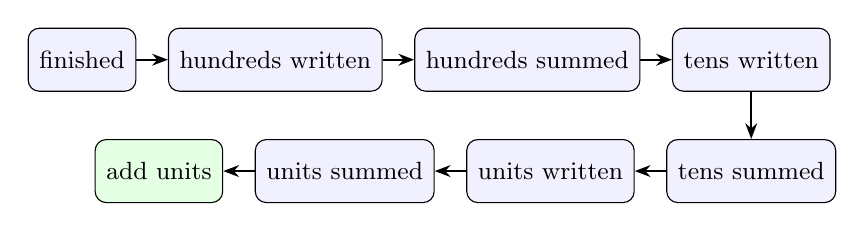
\begin{tikzpicture}[node distance=4mm, every node/.style={font=\small}]
    \node[box] (f) {finished};
    \node[box, right=of f] (w2) {hundreds written};
    \node[box, right=of w2] (s2) {hundreds summed};
    \node[box, right=of s2] (w1) {tens written};
    \node[box, below=6mm of w1] (s1) {tens summed};
    \node[box, left=of s1] (w0) {units written};
    \node[box, left=of w0] (s0) {units summed};
    \node[box, left=of s0, fill=green!10] (a0) {add units};
    \draw[arr] (f) -- (w2); \draw[arr] (w2) -- (s2); \draw[arr] (s2) -- (w1);
    \draw[arr] (w1) -- (s1); \draw[arr] (s1) -- (w0); \draw[arr] (w0) -- (s0); \draw[arr] (s0) -- (a0);
  \end{tikzpicture}
  \end{center}
  \begin{itemize}
    \item The goal names no order: only \emph{finished}. Finishing needs the hundreds written; writing needs the sum; adding a column needs the column to its right written, for its carry.
    \item Subgoaling works back to the units column, and the work runs units, tens, hundreds.
    \item GPS gives the right answers (15+17, 999+1, 478+256), by evaluation.
  \end{itemize}
\end{frame}
\note{
Here's the first result. GPS's goal is only to be finished; nothing says to start with the units. Finishing needs the hundreds written. Writing a column needs its sum. And adding a column needs the column to its right written, because that's where its carry comes from. So subgoaling works backward until it reaches the units column, the only column with no prerequisite, and the work then runs units, tens, hundreds. The right-to-left order of the algorithm falls out of the preconditions. On the problems I've run, GPS gets the right answers; a proof for every problem is still to do.
}

\begin{frame}{The bridge: the solver is the column backup}
  \begin{itemize}
    \item The multi-digit model's backup, \code{columns}, was a fixed procedure: units, tens, hundreds, with carrying written in.
    \item \textbf{Proved}: the problem solver with the full procedure answers \emph{exactly} as \code{columns} does, for every problem and every single-digit process.
    \item So the solver \textbf{replaces} the backup, and every multi-digit theorem about it still holds: carrying adds no error; a column error is a single-digit error moved to its place; confident errors.
  \end{itemize}
  \medskip
  The proof regroups the solver's step-by-step chain of draws into the backup's three nested draws (associativity of probabilistic composition), then checks place value.
\end{frame}
\note{
The second result is a bridge. The multi-digit model's backup used to be a fixed procedure, columns with carrying written in. With the full procedure, the problem solver gives exactly the same distribution of answers, for every problem and every single-digit process. So it replaces the backup, and nothing proved before is lost: carrying adds no error, a column error is a single-digit error moved to its place, and the confident-error results stand. The proof regroups the solver's one-step-at-a-time chain into the backup's three nested draws, and then it's place value.
}

\begin{frame}{Delete the carry rule}
  \begin{itemize}
    \item Without the carry rule, the procedure tries to \emph{write} every column sum.
    \item A sum of 10 or more violates \emph{write}'s precondition: an \textbf{impasse}.
    \item \textbf{Proved}: a problem whose columns all sum to less than 10 is still answered \emph{exactly}, whatever the repairs. No impasse arises.
  \end{itemize}
  \bigskip
  So a learner without carrying looks competent on every no-carry problem. Only carry problems reveal what is missing.
\end{frame}
\note{
Now delete the carry rule, as repair theory does to model incomplete learning. The procedure tries to write every column's sum, and a sum of ten or more violates write's precondition. That's an impasse. A first theorem: if no column sums to ten or more, the answer is exact, whatever the repairs, because no impasse ever arises. So this learner looks fully competent on every problem that doesn't need a carry. Only carry problems reveal what's missing, which is why diagnostic tests need them.
}

\begin{frame}{Four repairs, four bugs}
  \begin{center}
  \begin{tabular}{llc}
    \toprule
    Repair at the impasse & $15 + 17$ answered & probability\\
    \midrule
    Skip (blank cell) & 20 & $1/4$\\
    Quit & 0 & $1/4$\\
    Write the units digit only & 22 (no carry) & $1/4$\\
    Write both digits & 212 & $1/4$\\
    \midrule
    full procedure & 32 & 1\\
    \bottomrule
  \end{tabular}
  \end{center}
  \begin{itemize}
    \item Repair theory's heuristics, carried over from subtraction, generate addition bugs, the no-carry bug among them.
    \item With no critics, the repair is chosen at random: a distribution over bugs.
  \end{itemize}
\end{frame}
\note{
At the impasse, the four repairs give four bugs. On fifteen plus seventeen, skipping the cell leaves the units blank, giving twenty; quitting gives nothing; writing only the units digit gives twenty-two, the familiar forgot-to-carry answer; and writing both digits in the units cell gives two hundred twelve. With no critics, each happens a quarter of the time. Brown and VanLehn's heuristics were designed for subtraction; carried over unchanged, they generate addition bugs, including the familiar no-carry one, which is the kind of domain-independence they hoped for.
}

\begin{frame}{Critics select the bug}
  \begin{itemize}
    \item Critics against blank cells, quitting, and two digits in a cell leave one repair: write the units digit.
    \item \textbf{Proved, for every problem}: the answer is the columns added without carrying,
    \[
      \textstyle\sum_{i} \big((a_i + b_i) \bmod 10\big)\cdot 10^i.
    \]
  \end{itemize}
  \bigskip
  A learner's bug is a joint product of what is missing (the carry rule) and what they will not do (the critics). A stable bug is predicted where the critics leave a single repair.
\end{frame}
\note{
Critics narrow the choice. A learner who won't leave a cell blank, won't give up, and won't put two digits in a cell has only one repair left: write the units digit. Then, for every problem, the answer is each column's sum without carrying. That's proved in general, not checked on examples. So a bug is the joint product of what the learner is missing, the carry rule, and what they won't do, their critics. Where the critics leave a single repair, the theory predicts a stable bug; where they leave several, the same learner can answer the same problem in different wrong ways.
}

\begin{frame}{What is proved, and what is not yet}
  \small
  \begin{tabular}{p{0.45\linewidth}p{0.45\linewidth}}
    \toprule
    For every problem / setting & On examples, or not yet\\
    \midrule
    Impasse $\iff$ violated precondition & GPS's answers (three problems)\\
    The bridge to \code{columns} & Soar's tie and conflict impasses\\
    No-carry learner exact without carries & Chunking (next)\\
    The no-carry bug under strict critics & Subtraction, repair theory's own domain\\
    \bottomrule
  \end{tabular}
\end{frame}
\note{
To be clear about what's proved. In general: an impasse is exactly a violated precondition; the bridge to the column backup, for every problem and process; exactness without carries; and the no-carry bug under strict critics, for every problem. On examples only: GPS's answers, on three problems; a general GPS theorem is next. Not yet: Soar's other impasse types, chunking, and subtraction, which is repair theory's own domain.
}

\begin{frame}{Next}
  \begin{itemize}
    \item \textbf{Chunking} (Soar): the result of a subgoal becomes a new rule. In addition, a fact found by counting at a retrieval impasse becomes an association: DOA's own learning rule, seen from the problem-solving side.
    \item A general GPS theorem: units-first and exact, for every problem.
    \item \textbf{Subtraction} and borrowing, where repair theory's bug data are.
    \item Laws comparing the regimes, matrix-style: \emph{every subgoal arises from an impasse}, \emph{learning only by chunking}, \dots
  \end{itemize}
\end{frame}
\note{
Next. Chunking, Soar's learning mechanism, where the result of a subgoal becomes a new rule. In addition, when retrieval reaches an impasse and the fact is found by counting, chunking would store it as an association, which is exactly the distributions-of-associations model's learning rule, seen from the problem-solving side. A general GPS theorem. Subtraction and borrowing, where repair theory's own bug data are. And laws that separate the control regimes, so that GPS and Soar get rows in a matrix like the memory families.
}

\end{document}
